\section{Explicaci\'o del codi}

\subsection{HomeController}
El fitxer HomeController.cs \'es l'encarregat de manegar la web.
T\'e una funci\'o per cada p\`agina`,
que prepara la vista d'aquesta i mostra l'html resultant al client.
Dep\`en de la funci\'o executada, carrega una vista o una altra,
que t\'e el mateix nom que la funci\'o.


\subsection{Trucades a la api}
Per aconseguir els valors per mostrar a la p\`agina,
primer es fa una trucada a l'api des de HomeController.cs
(aquesta dep\`en de la p\`agina que est\`a carregant i l'argument que ha rebut).

\begin{figure}[!h]
	\centering
	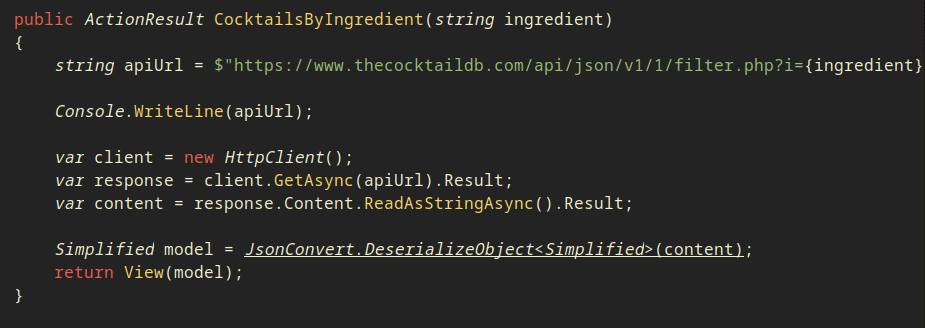
\includegraphics[width=0.8\columnwidth]{homecontroller-ex.png}
	\caption{Exemple de funci\'o a HomeController.cs}
\end{figure}

Els resultats de la trucada s\'on rebuts en format JSON,
que es transforma utilitzant Newtonsoft per guardar-se en la variable model,
que \'es una inst\`ancia d'una classe amb els par\`ametres que es volen mostrar
i s'utilitza com a argument al carregar la vista.
En el nostre cas, les classes s\'on llistes amb informaci\'o sobre
les begudes que es volen mostrar.

\begin{figure}[!h]
	\centering
	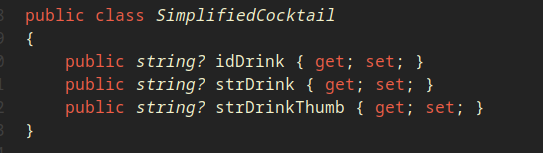
\includegraphics[width=0.8\columnwidth]{simplifiedcocktail.png}
	\caption{Exemple de classe a Cocktail.cs}
\end{figure}


\subsection{Vistes}
Per carregar la vista,
primer s'executen tamb\'e els arxius \_ViewStart.cs i \_ViewImport.cs
per carregar els layouts corresponents i importar els m\`oduls necessaris.

Les vistes s\'on l'html rebut per part del controlador,
que \'es el que es mostra a la pantalla del client.
Aquests es fan a partir dels fitxers cshtml,
que ajunten html amb funcions de C\# i ASP.

Algunes d'aquestes funcions utilitzades s\'on el foreach,
que repeteix un codi html per cada beguda que es vulgui mostrar,
o un if, per comprovar condicions.
Tamb\'e s'utilitzen variables per mostrar par\`ametres a l'html,
com ara la informaci\'o de les begudes mostrades
(incluint t\'itol, descripci\'o, imatge...).

\begin{figure}[!h]
	\centering
	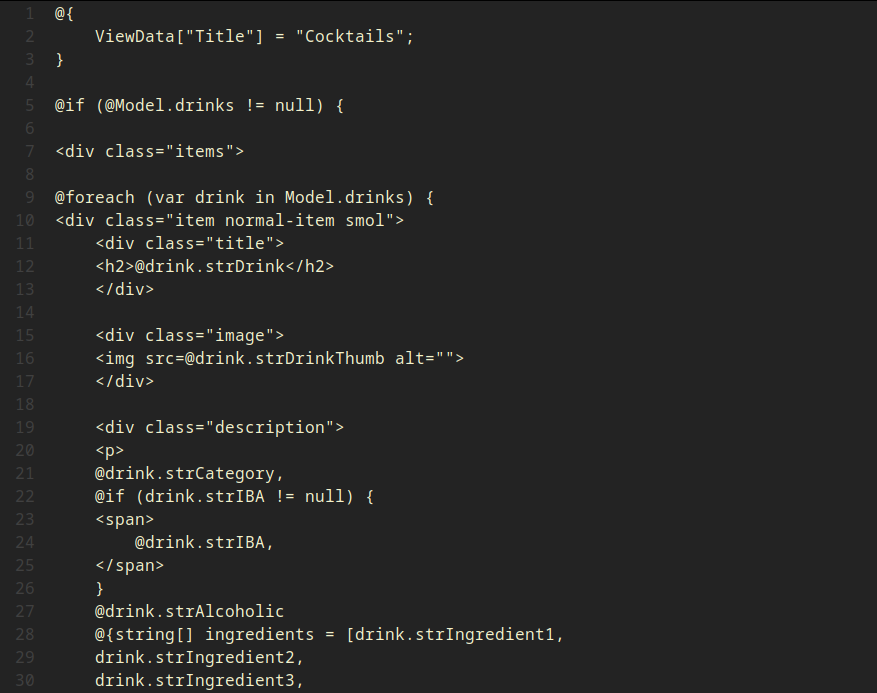
\includegraphics[width=0.8\columnwidth]{cshtml-ex.png}
	\caption{Exemple de cshtml a Cocktails.cshtml}
\end{figure}

Els fitxers de la carpeta home utilitzen comparteixen el codi del layout,
que s'afegeix autom\`aticament a totes les vistes.
Aquest cont\'e configuracions del head, el t\'itol, el navbar i la barra de busca.
\'Es un fitxer compartit per no haver de repetir aquella porci\'o de codi a cada cshtml.

\begin{figure}[!h]
	\centering
	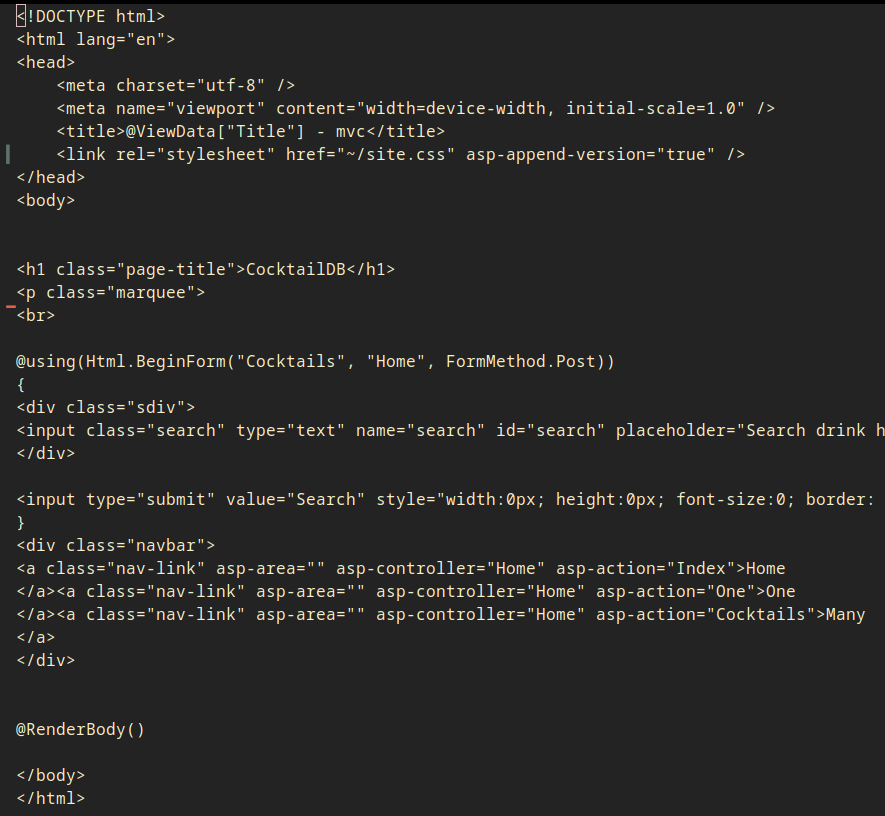
\includegraphics[width=0.8\columnwidth]{cshtml-layout-cut.png}
	\caption{\_Layout.cshtml (tallat)}
\end{figure}

\subsection{Links}
Per anar de p\`agina en p\`agina,
s'utilitzen links amb par\`ametres especials (de cshtml)
que truquen a altres funcions de HomeController.
Per cada funci\'o, es carrega la vista amb aquest mateix nom.
En cas de que requereixin m\'es informaci\'o,
com ara els valors que es volen buscar (com a argument),
s'utilitza asp-target per canviar-los.

D'una manera similar funciona el formulari,
al qual se l'ha d'especificar a quina funci\'o est\`a trucant,
i aquest retornar\'a els valors del formulari en forma d'argument.
Els formularis s\'on utilitzats per fer funcionar la barra de busca.
